\documentclass[xcolor=dvipsnames]{beamer}
\usecolortheme[named=Green]{structure}
\usetheme{Boadilla}
\begin{document}
\author{Matthew Via and Victoria Chwalowski}
\title{Patrick Stewart}
\date{\today}
\newtheorem{fct}{Fact}
\newtheorem{qct}{Quote}
\begin{frame}{}
  \begin{columns}
    \begin{column}{0.5\textwidth}
      \titlepage
    \end{column}
    \begin{column}{0.5\textwidth}
      \begin{center}
        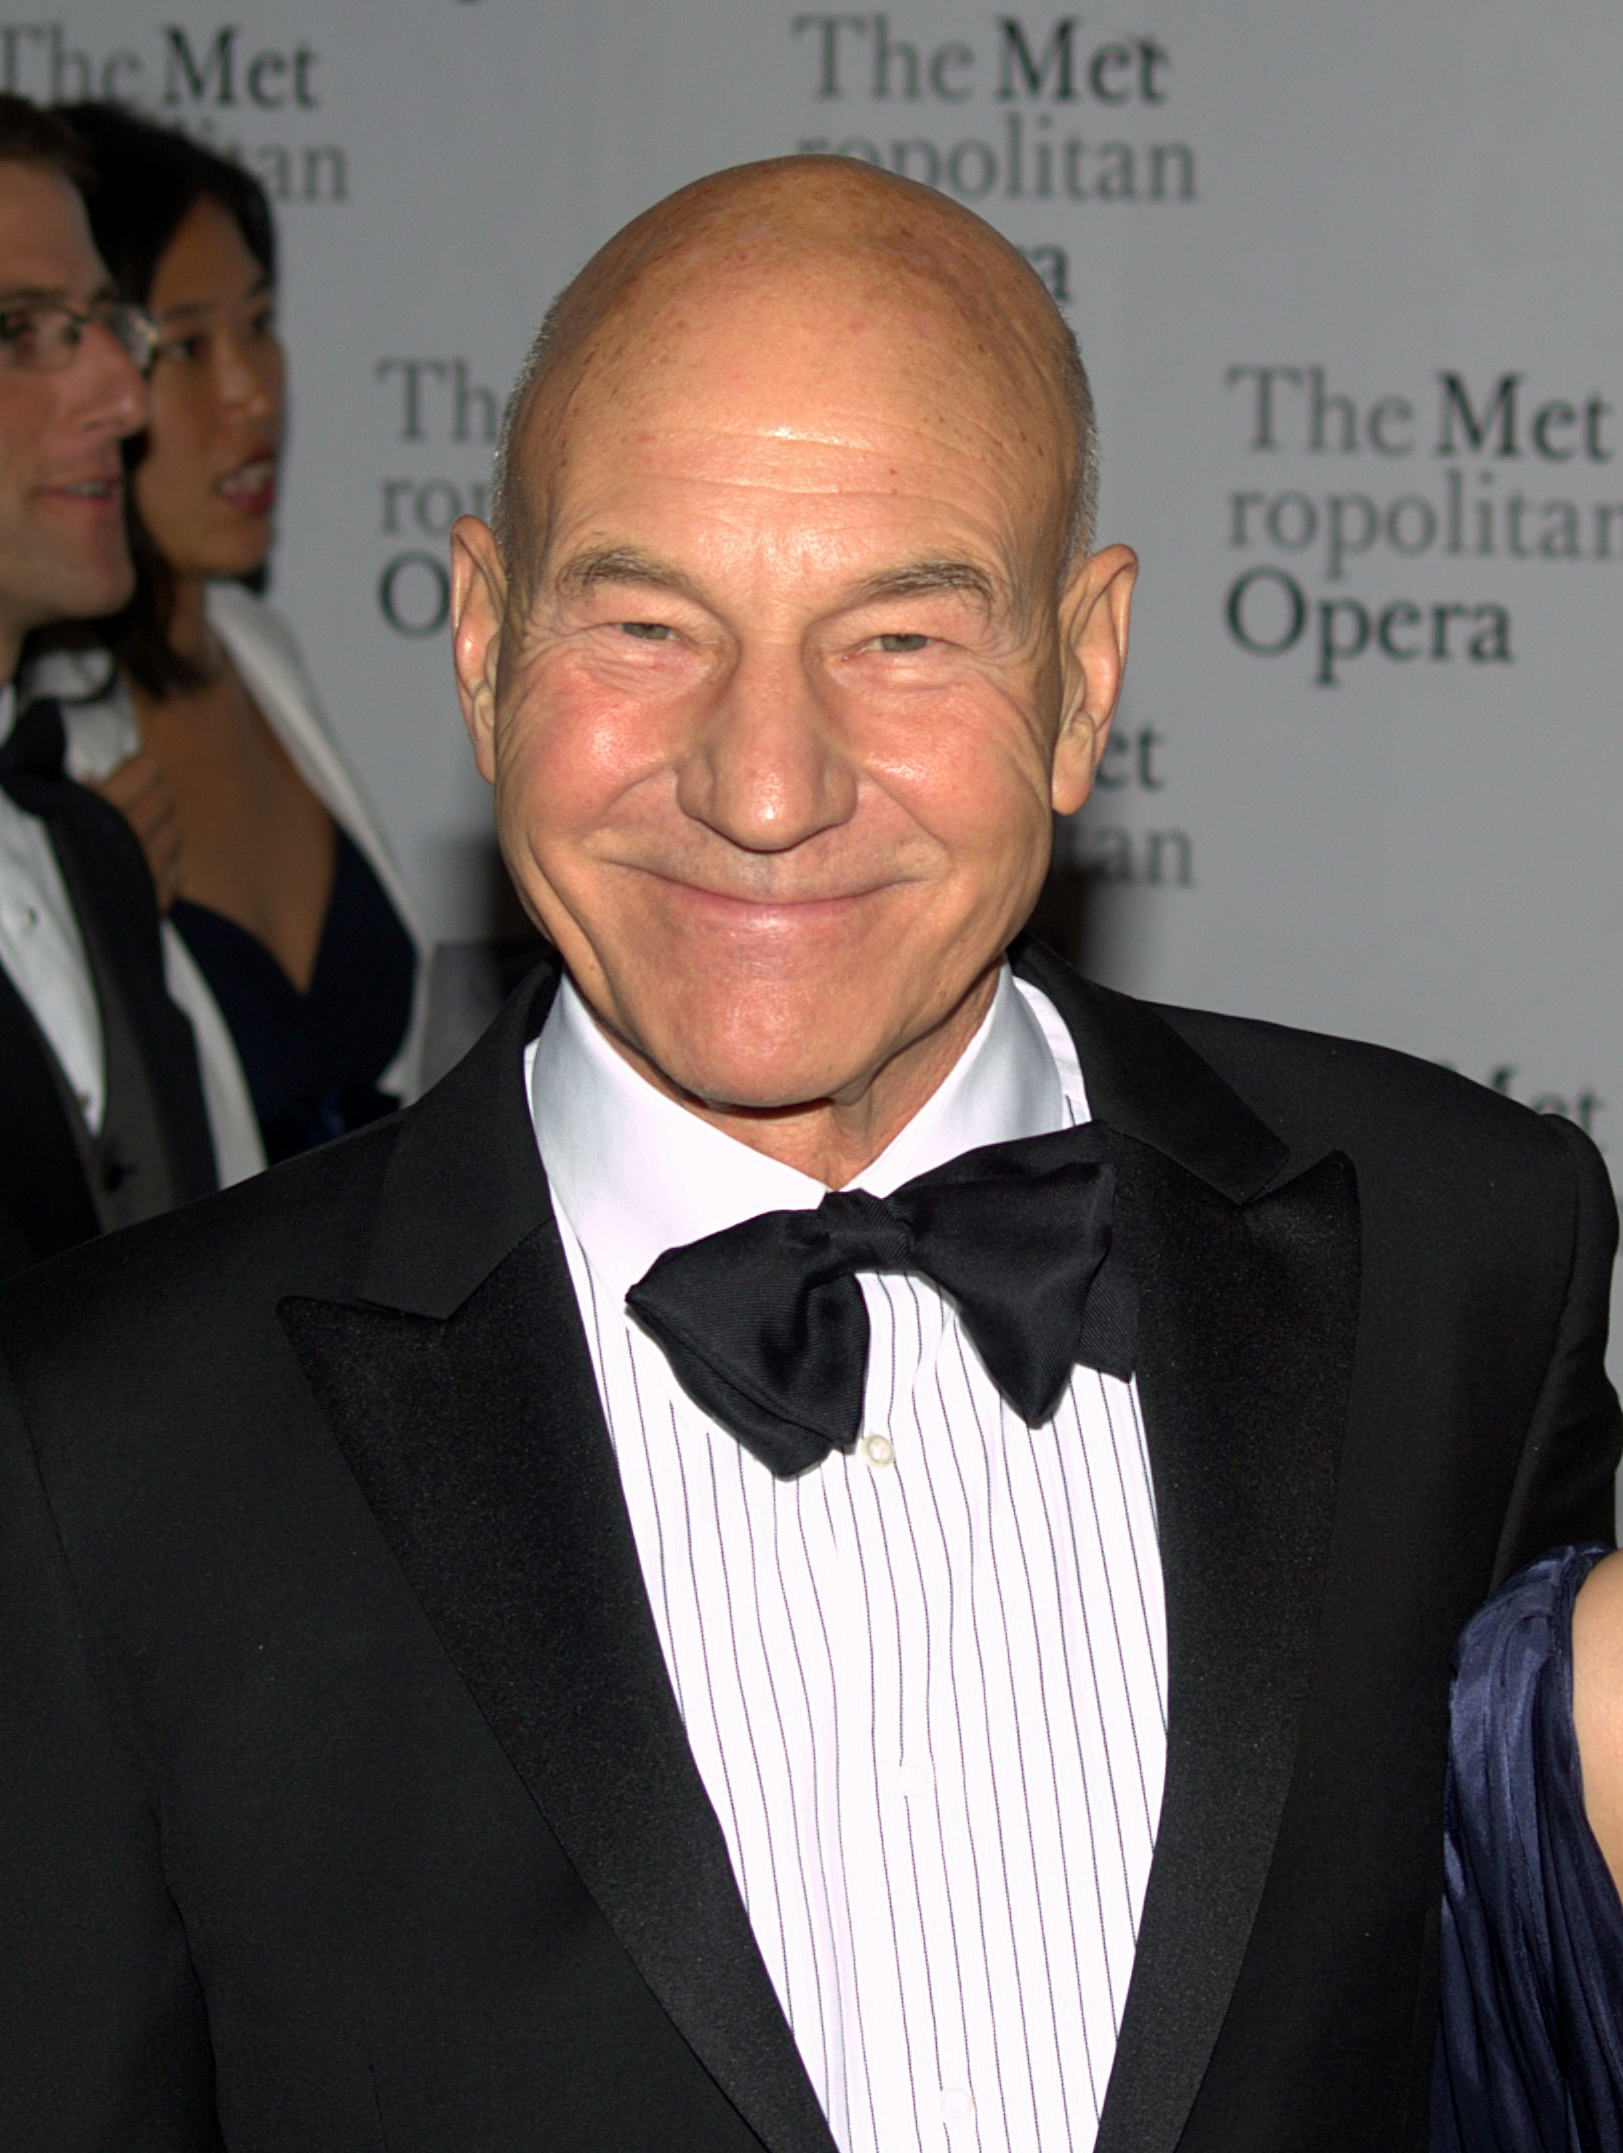
\includegraphics[width=0.8\textwidth]{smile.jpg}
      \end{center}
    \end{column}
  \end{columns}
\end{frame}

\begin{frame}{Early life}
  \begin{fct}
    Sir Patrick Stewart was born on 13 July 1940.
  \end{fct}
  \begin{itemize}
    \item Born to Gladys and Alfred Stewart
    \begin{itemize}
      \item Mother worked with textiles
      \item Father worked as general labourer and postman
      \item Father was a Regimental Sergeant Major in the British Army
    \end{itemize}
    \item Heavily influenced by his fathers strong will
    \item Grew up in poverty, affecting his later political beliefs
  \end{itemize}
  \begin{center}
    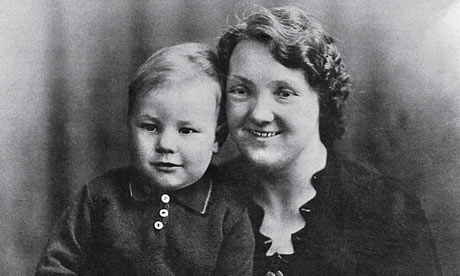
\includegraphics[width=0.3\textwidth]{kid.jpg}
  \end{center}
\end{frame}

\begin{frame}{Early Career}
  \begin{itemize}
    \item Dropped out of school at age 15 and got a job as a journalist
    \item Increased involvement in local theater
    \item After a year, quit journalism and decided to go to acting school
    \item Became a furniture salesman while saving money for Bristol Old Vic
    Acting School
  \end{itemize}
  \begin{fct}
    Sir Patrick Stewart lost his hair at age 19.
  \end{fct}
\end{frame}

\begin{frame}{Early Theatre Work}
  \begin{itemize}
    \item Joined the Manchester Library Theatre
    \item 1959 debut as Morgan in a stage adaptation of Treasure Island
    \item Several brief appearances on British television (\emph{Coronation
    Stree} and \emph{Civilisation})
    \item First major television appearance in 1974 as Lenin in \emph{Fall of Eagles}
  \end{itemize}
\end{frame}

\begin{frame}{Shakespeare Influence}
  \begin{itemize}
    \item Member of Royal Shakespeare Company in 1966, Associate Artist with the Company in 1968
    \item Made Broadway debut as Snout in \emph{A Midsummer's Night Dream}
    \begin{qct}
      \emph{We were, all of us, dazzled by the enthusiasm that the audience
      brought. Until the Macbeth, it was probably the biggest smash I had ever
      been in.}
    \end{qct}
    \item Appeared in over 60 productions, most recently \emph{Hamlet} in 2008
  \end{itemize}
\end{frame}

\begin{frame}{Star Trek: TNG}

\end{frame}

\begin{frame}{X-Men}
  \begin{columns}
    \begin{column}{0.7\textwidth}
      \begin{itemize}
        \item Probably his most well known acting career, Stewart played the role of Professor
        Xavier in the X-Men series, including:
        \begin{itemize}
          \item{\emph{X-Men}}
          \item{\emph{X2}}
          \item{\emph{X-Men: The Last Stand}}
        \end{itemize}
        \item Also did voice acting for three X-Men based video games afterwards
        \item Developed a close friendship with Ian McKellen on the set
      \end{itemize}
    \end{column}
    \begin{column}{0.3\textwidth}
      
\includegraphics[width=0.8\textwidth]{xavier.jpg}
    \end{column}
  \end{columns}

\end{frame}

\begin{frame}{A Christmas Carol}

\end{frame}

\begin{frame}{Other Films}
  \begin{itemize}
    \item 1984: Played Gurney Halleck in David Lynch's \emph{Dune}
  \end{itemize}
\end{frame}

\begin{frame}{Voice Acting}
  \begin{columns}
    \begin{column}{0.7\textwidth}
      \begin{itemize} 
        \item 2005-2010: Avery Bullock on \emph{American Dad}
      \end{itemize}
    \end{column}
    \begin{column}{0.3\textwidth}
      
\includegraphics[width=0.9\textwidth]{Bullock.jpg}
    \end{column}
  \end{columns}
\end{frame}

\begin{frame}{Personal Life}

\end{frame}

\begin{frame}{Political Beliefs}
  Stewart's general beliefs can be summarized as fairness and equality.  
  \begin{itemize}
    \item Opposed the Iraq War
    \item Critized government for extending detention without charge to 42
    days, and signed a letter of objection to it.
    \item Advocates for legalization of assisted suicide
  \end{itemize}
  His childhood as a lower class citizen gave him perspective on social issues.

\end{frame}

\begin{frame}{Awards Received}
  \begin{itemize}
    \item 2 July 2010: Awarded Knighthood by Queen of England
    \item 1992: Awarded "Sexiest Man on Television" by TV Guide
  \end{itemize}
\end{frame}
\begin{frame}{About this Presentation}
  This presentation was produced using only open-source software.

  The slides were created using Beamer and LaTeX, and group collaboration was done
  with git.
\end{frame}
\end{document}
